% \documentclass[letterpaper]{article} % DO NOT CHANGE THIS
% \usepackage{aaai24}  % DO NOT CHANGE THIS
% \usepackage{times}  % DO NOT CHANGE THIS
% \usepackage{helvet}  % DO NOT CHANGE THIS
% \usepackage{courier}  % DO NOT CHANGE THIS
% \usepackage[hyphens]{url}  % DO NOT CHANGE THIS
% \usepackage{graphicx} % DO NOT CHANGE THIS
% \urlstyle{rm} % DO NOT CHANGE THIS
% \def\UrlFont{\rm}  % DO NOT CHANGE THIS
% \usepackage{natbib}  % DO NOT CHANGE THIS AND DO NOT ADD ANY OPTIONS TO IT
% \usepackage{caption} % DO NOT CHANGE THIS AND DO NOT ADD ANY OPTIONS TO IT
% \frenchspacing  % DO NOT CHANGE THIS
% \setlength{\pdfpagewidth}{8.5in}  % DO NOT CHANGE THIS
% \setlength{\pdfpageheight}{11in}  % DO NOT CHANGE THIS


% % Keep the \pdfinfo as shown here. There's no need
% % for you to add the /Title and /Author tags.
% \pdfinfo{
% /TemplateVersion (2024.1)
% }



% \usepackage{subcaption}
% \usepackage{amsmath}
% \usepackage{amssymb}
% \usepackage{mathtools}
% \usepackage{amsthm}

% \usepackage[utf8]{inputenc} % allow utf-8 input
% \usepackage{booktabs}       % professional-quality tables
% \usepackage{amsfonts}       % blackboard math symbols
% \usepackage{nicefrac}       % compact symbols for 1/2, etc.
% \usepackage{microtype}      % microtypography
% \usepackage{xcolor}         % colors

% \DeclareMathOperator*{\argmax}{arg\,max}
% \DeclareMathOperator*{\argmin}{arg\,min}
% \DeclareMathOperator*{\clip}{clip}

% \newtheorem{definition}{Definition}
% \newtheorem{lemma}{Lemma}
% \newtheorem{theorem}{Theorem}

% % \usepackage[textsize=tiny]{todonotes}
% \newcommand{\omer}[1]{{\color{red}{Omer: #1}}}

% \setcounter{secnumdepth}{1} %May be changed to 1 or 2 if section numbers are desired; the default is 0


% \setcounter{figure}{4}

% % Title

% % Your title must be in mixed case, not sentence case.
% % That means all verbs (including short verbs like be, is, using,and go),
% % nouns, adverbs, adjectives should be capitalized, including both words in hyphenated terms, while
% % articles, conjunctions, and prepositions are lower case unless they
% % directly follow a colon or long dash
% \title{Personalized Reinforcement Learning with a Budget of Policies\\Appendix}

% \author{
%     Dmitry Ivanov,
%     Omer Ben-Porat
% }

% \affiliations{
%     Technion, Israel\\
%     divanov@campus.technion.ac.il, omerbp@technion.ac.il
% }



% \begin{document}

% \maketitle


\appendix



\section{Convergence of the EM-like Algorithm}

We use notations from Section 2 of the main text.

The objective is to maximize utilitarian social welfare:

$$SW(\boldsymbol\alpha, \boldsymbol\pi) = \mathbb{E}_{\mathcal{T}_0} \sum_{i, j} \alpha^i(j) V^{ij}(s_0),$$

\noindent where $\boldsymbol\alpha = (\alpha^i)_{i \in N}$ and $\boldsymbol\pi = (\pi^{j})_{j \in K}$.

% The objective is to maximize utilitarian social welfare:

% $$\max_{(\alpha^i)_{i \in N}, (\pi^{j})_{j \in K}} \mathbb{E}_{\mathcal{T}_0} \sum_{i, j} \alpha^i(j) V^{ij}(s_0),$$

% \noindent or, equivalently:

% $$\max_{(\pi^{j})_{j \in K}} \mathbb{E}_{\mathcal{T}_0} \sum_{i} \max_{j \in K} V^{ij}(s_0).$$

% Let $\boldsymbol\pi = (\pi^{j})_{j \in K}$. Denote the social welfare as:

% $$SW(\boldsymbol\pi) = \mathbb{E}_{\mathcal{T}_0} \sum_{i} \max_{j \in K} V^{ij}(s_0).$$

\begin{lemma}\label{lemma:app}
    A function $V^j$ defined by $V^j(s) = \sum_{i \in N} \alpha^i(j) V^{ij}(s)$ is a value function.
\end{lemma}

\begin{proof}
    Let $s \in S$.
    
    Apply the definition of $V^{ij}(s)$:
    
    $$
    V^j(s) = \sum_{i \in N} \alpha^i(j) \mathbb{E} \left[ \overset{T}{\underset{t=0}{\sum}} \gamma^{t} \tilde{r}^i_t \mid s_0 = s, \pi^j \right].
    $$

    Rearrange the terms:

    $$
    V^j(s) = \mathbb{E} \left[ \overset{T}{\underset{t=0}{\sum}} \gamma^{t} \sum_{i \in N} \alpha^i(j) \tilde{r}^i_t \mid s_0 = s, \pi^j \right].
    $$

    Substitute $\tilde{r}^j_t = \sum_{i \in N} \alpha^i(j) \tilde{r}^i_t$:

    $$
    V^j(s) = \mathbb{E} \left[ \overset{T}{\underset{t=0}{\sum}} \gamma^{t} \tilde{r}^j_t \mid s_0 = s, \pi^j \right].
    $$

    Observe that $V^j(s)$ is a value function by definition.
\end{proof}

% A corollary of Lemma \ref{lemma:app} is that we can use any RL algorithm to find an optimal policy $\pi^j$ given fixed assignments.


Define the \textit{E-step} as updating the assignments to $\boldsymbol\alpha^*$ given the policies $\boldsymbol\pi$:

\begin{equation}
    \alpha^{i*}(j^*) = 
    \begin{dcases}
        1,& j^* = \argmax_j \mathbb{E}_{\mathcal{T}_0} V^{ij}(s_0)\\
        0,              & \text{otherwise}
    \end{dcases}
\end{equation}

\noindent Note: ties are broken arbitrarily, e.g., lexicographically.


Define the \textit{M-step} as updating the policies to $\boldsymbol\pi^*$ given the assignments $\boldsymbol\alpha$:

\begin{equation}
   \forall \{ j \mid \sum_i \alpha^i(j) > 0 \} : \pi^{j*} = \argmax_{\pi^j} \mathbb{E}_{\mathcal{T}_0} V^j(s_0)
\end{equation}

\noindent Note: if some representative $j$ is not assigned any agents after an E-step (i.e., $\sum_i \alpha^i(j) = 0$), we may assign a random agent to this representative prior to the M-step. After the M-step, the representative will implement the optimal policy for this agent. For the formal proof, this is not required.

By Lemma \ref{lemma:app}, we can use any RL algorithm that has convergence guarantees to perform the M-step for each $j$.


The EM-like meta-algorithm is defined in Algorithm \ref{alg:algorithm}. A specific implementation is discussed in the main text.

\begin{algorithm}[tb]
    \caption{EM-like meta-algorithm}
    \label{alg:algorithm}
    \textbf{Input}: r-MDP $\mathcal{M}_r$
    \begin{algorithmic}[1] %[1] enables line numbers
        \STATE Arbitrarily initialize $(\alpha^i)_{i \in N}$ s.t. $\forall j: \exists i, \alpha^i(j) > 0$
        \WHILE{assignments or policies change}
            \STATE Perform M-step to update policies
            \STATE Perform E-step to update assignments
        \ENDWHILE
    \end{algorithmic}
\end{algorithm}



\begin{theorem}\label{theorem:app}
    Given an r-MDP $\mathcal{M}_r$, the EM-like meta-algorithm converges to a local maximum of $SW(\boldsymbol\alpha, \boldsymbol\pi).$ 
\end{theorem}

\begin{proof}
    Observe that an E-step may not decrease social welfare:

    \begin{equation*}
    \begin{split}
        & SW(\boldsymbol\alpha^*, \boldsymbol\pi) - SW(\boldsymbol\alpha, \boldsymbol\pi) =\\
        & \mathbb{E}_{\mathcal{T}_0} \sum_i \left[ \max_j V^{ij}(s_0) - \sum_j \alpha^i(j) V^{ij}(s_0) \right] \geq 0.
    \end{split}
    \end{equation*}

    Likewise, observe that an M-step may not decrease social welfare:

    \begin{equation*}
    \begin{split}
        & SW(\boldsymbol\alpha, \boldsymbol\pi^*) - SW(\boldsymbol\alpha, \boldsymbol\pi) =\\
        & \mathbb{E}_{\mathcal{T}_0} \sum_{i, j} \left[ \alpha^i(j) \left( V^i(s_0 \mid \pi^{j*}) - V^i(s_0 \mid \pi^j) \right) \right] \geq 0.
    \end{split}
    \end{equation*}

    Therefore, the iterative application of E-step and M-step monotonically increases social welfare until convergence. Because the number of possible assignments is finite, the convergence is guaranteed.
\end{proof}


\section{Hyperparameters and Technical Details}

\paragraph{PPO}

The PPO algorithm updates the policy to minimize the following loss function:

\begin{equation}\label{eq:loss_ppo_actor}
    \begin{split}
    L(\theta) = - \sum_{t \in B} \min[\rho_\theta(s_t, a_t) \tilde{A}(s_t, a_t),& \\  \min(\max(\rho_\theta(s_t, a_t), 1-\epsilon), 1+\epsilon) \tilde{A}(s_t, a_t)]&
    \end{split} % \clip(\rho_\theta(s_t, a_t), 1-\epsilon, 1+\epsilon) 
\end{equation}

Our implementation of PPO is based on the PyTorch package \cite{paszke2019pytorch} for Python 3. We followed the procedure of \cite{shengyi2022the37implementation} to replicate the performance from the original paper \cite{schulman2017proximal}. Specifically, we implemented:

\begin{itemize}
    \item Orthogonal weight initialization;
    \item Generalized advantage estimation \cite{schulman2015high};
    \item Normalization of advantages over the batch (per policy);
    \item Entropy bonus to encourage exploration;
    \item Gradient norm clipping;
    \item Continuous actions via normal distributions plus reparameterization trick;
    \item State-independent log standard deviations as learnable parameters;
    \item Independent action components;
    \item Action clipping;
    \item Normalization and clipping of observations.
\end{itemize}

Actors and critics were both trained with ADAM optimizers \cite{kingma2014adam}. Furthermore, we used hyperparameters standard for MuJoCo environments:

\begin{itemize}
    \item Learning rate initialized at $0.0003$ and annealed throughout the training to $0.0001$;
    \item Entropy loss coefficient of $0.001$;
    \item GAE $\lambda = 0.95$;
    \item One hidden layer with 64 neurons;
    \item Batch of 2048 transitions, divided into mini-batches of 64 transitions;
    \item A batch is used for training for 10 epochs;
    \item PPO clipping parameter $\epsilon = 0.2$;
    \item ADAM $\epsilon = 10^{-5}$.
\end{itemize}

\paragraph{Our algorithms}

For our EM-like algorithm, we used a mixing coefficient $\lambda = 0.05$. For our end-to-end algorithm, we updated $\psi$ with ADAM optimizer with a learning rate of $0.002$ in the same backward passes as the policies $\theta_i$.



\section{Additional Histograms}


Figure \ref{fig:results_histograms_app} reports histograms of assignments learned by ours and baseline algorithms. These echo the conclusions in the main text: our algorithms divide the latent velocity space better than the baseline, and thus provide more personalization.


\begin{figure*}[t]
\begin{center}
    \begin{subfigure}{0.3\textwidth}
        \centering
        \caption{Ant, EM (ours)}
        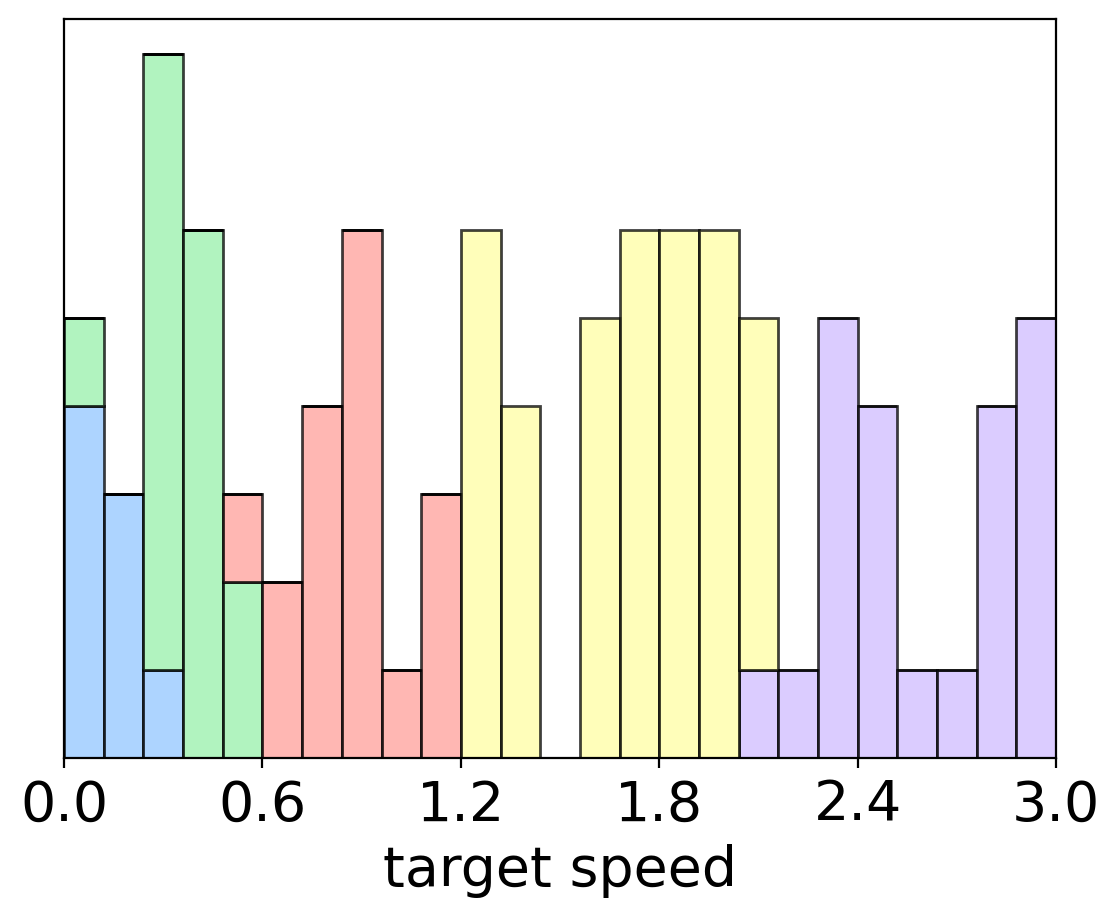
\includegraphics[width=\linewidth]{pics/histograms/em/Ant.png}
    \end{subfigure}\hspace{10pt}%
    \begin{subfigure}{0.3\textwidth}
        \centering
        \caption{Ant, end-to-end (ours)}
        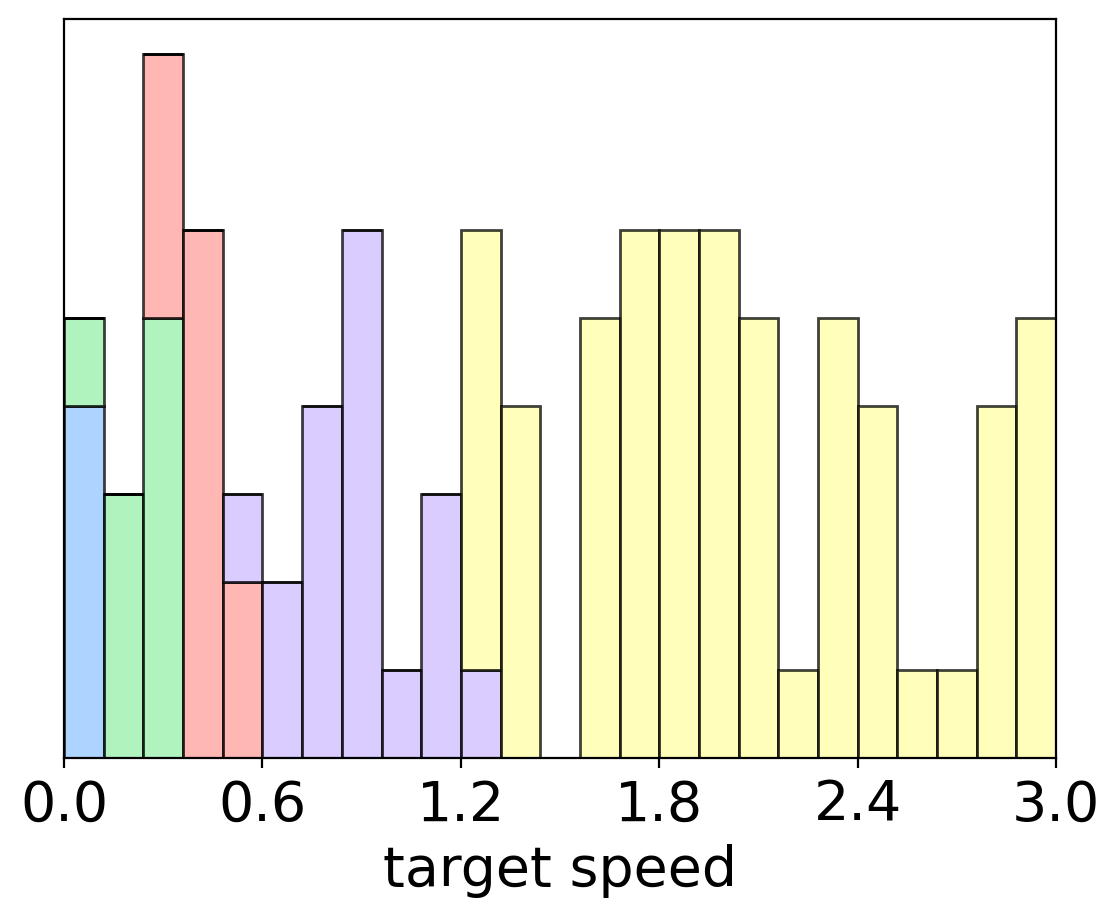
\includegraphics[width=\linewidth]{pics/histograms/end-to-end/Ant.png}
    \end{subfigure}\hspace{10pt}%
    \begin{subfigure}{0.3\textwidth}
        \centering
        \caption{Ant, cluster (baseline)}
        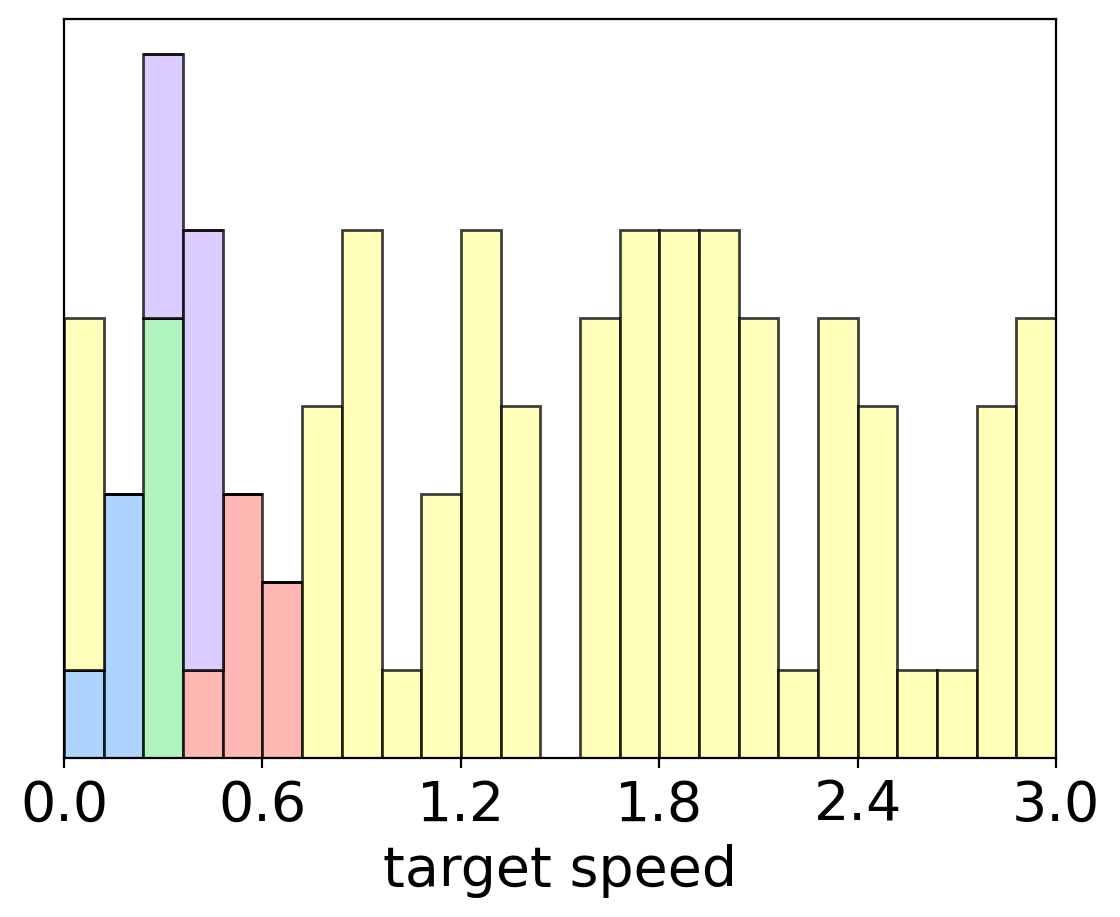
\includegraphics[width=\linewidth]{pics/histograms/cluster/Ant.png}
    \end{subfigure}
    
    \begin{subfigure}{0.3\textwidth}
        \centering
        \caption{Hopper, EM (ours)}
        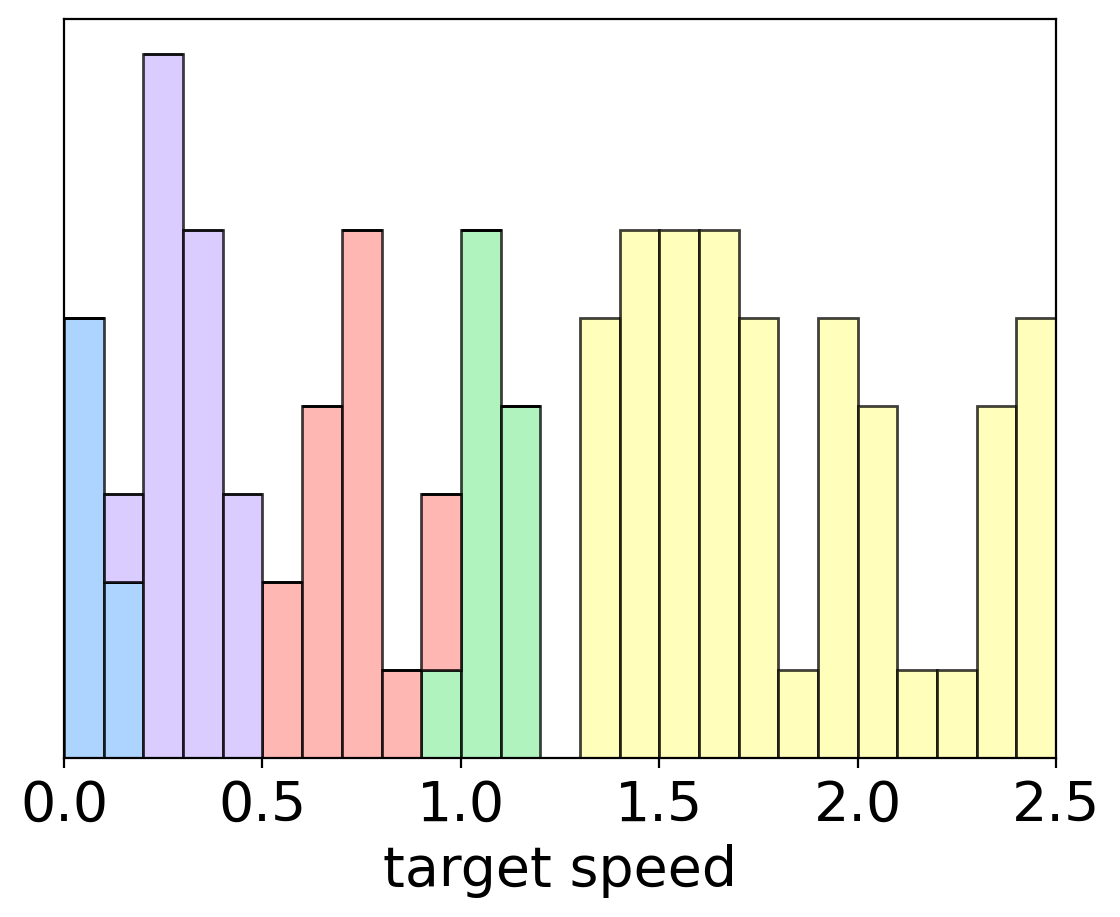
\includegraphics[width=\linewidth]{pics/histograms/em/Hopper.png}
    \end{subfigure}\hspace{10pt}%
    \begin{subfigure}{0.3\textwidth}
        \centering
        \caption{Hopper, end-to-end (ours)}
        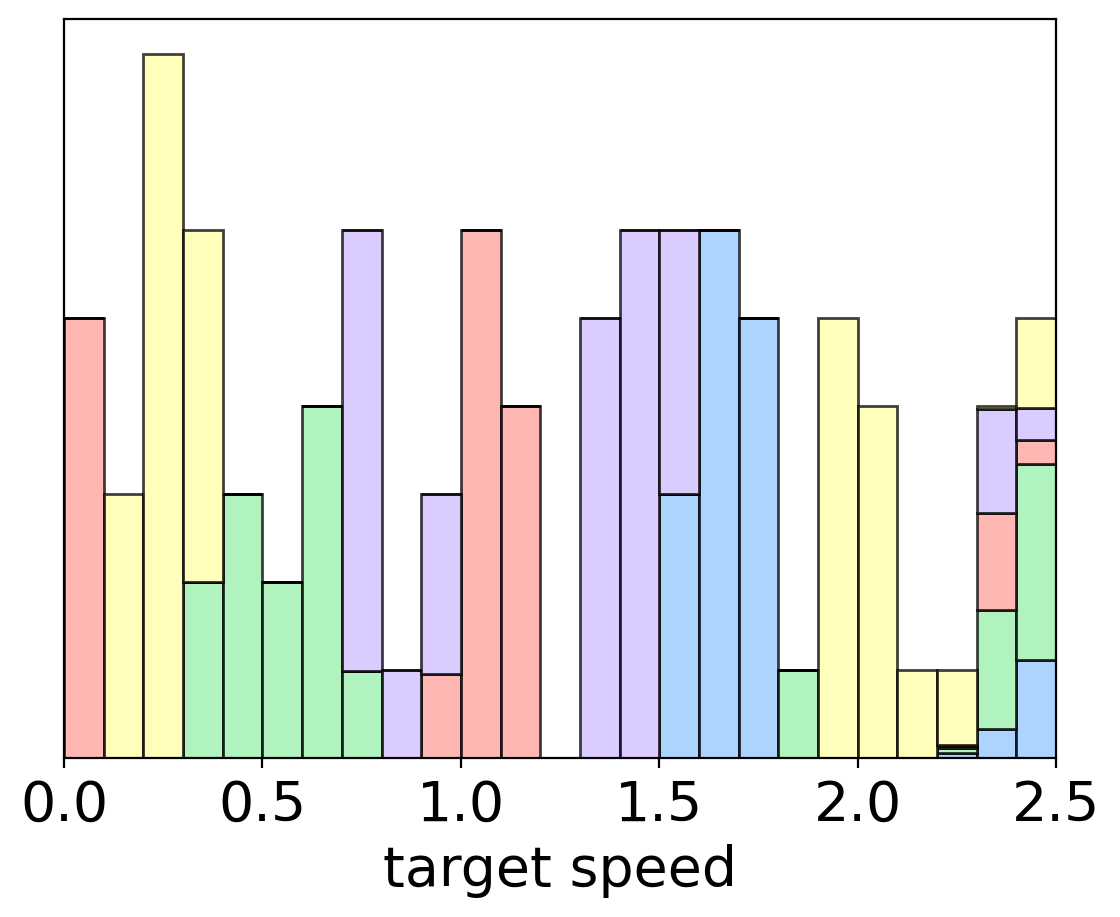
\includegraphics[width=\linewidth]{pics/histograms/end-to-end/Hopper.png}
    \end{subfigure}\hspace{10pt}%
    \begin{subfigure}{0.3\textwidth}
        \centering
        \caption{Hopper, cluster (baseline)}
        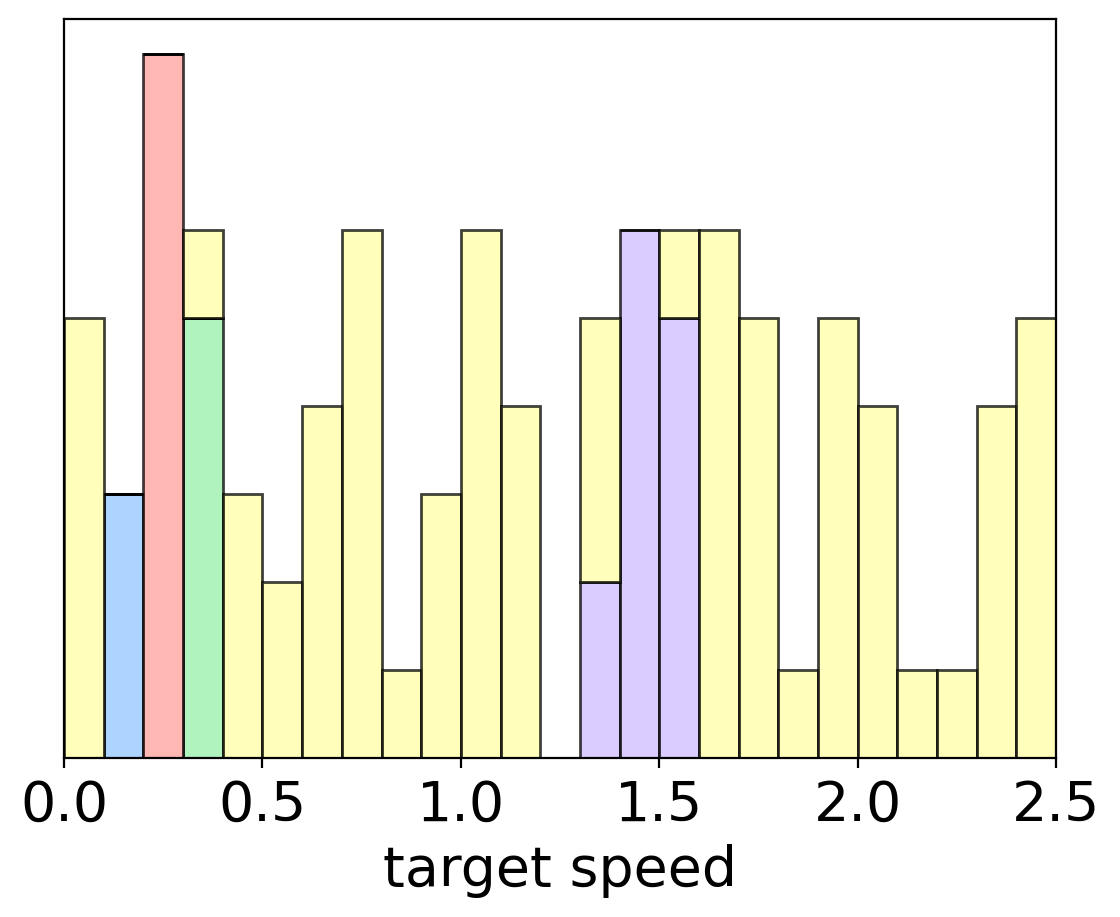
\includegraphics[width=\linewidth]{pics/histograms/cluster/Hopper.png}
    \end{subfigure}
    
    \begin{subfigure}{0.3\textwidth}
        \centering
        \caption{Walker2d, EM (ours)}
        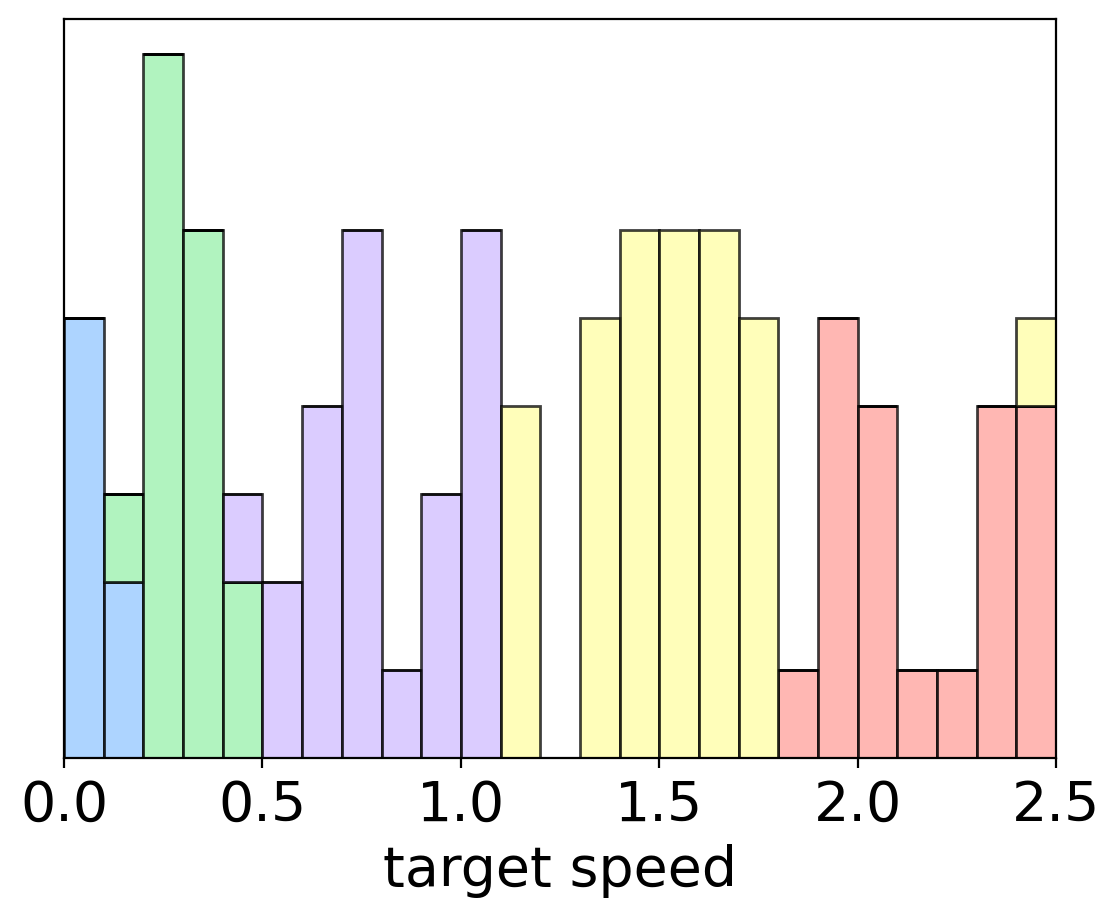
\includegraphics[width=\linewidth]{pics/histograms/em/Walker2d.png}
    \end{subfigure}\hspace{10pt}%
    \begin{subfigure}{0.3\textwidth}
        \centering
        \caption{Walker2d, end-to-end (ours)}
        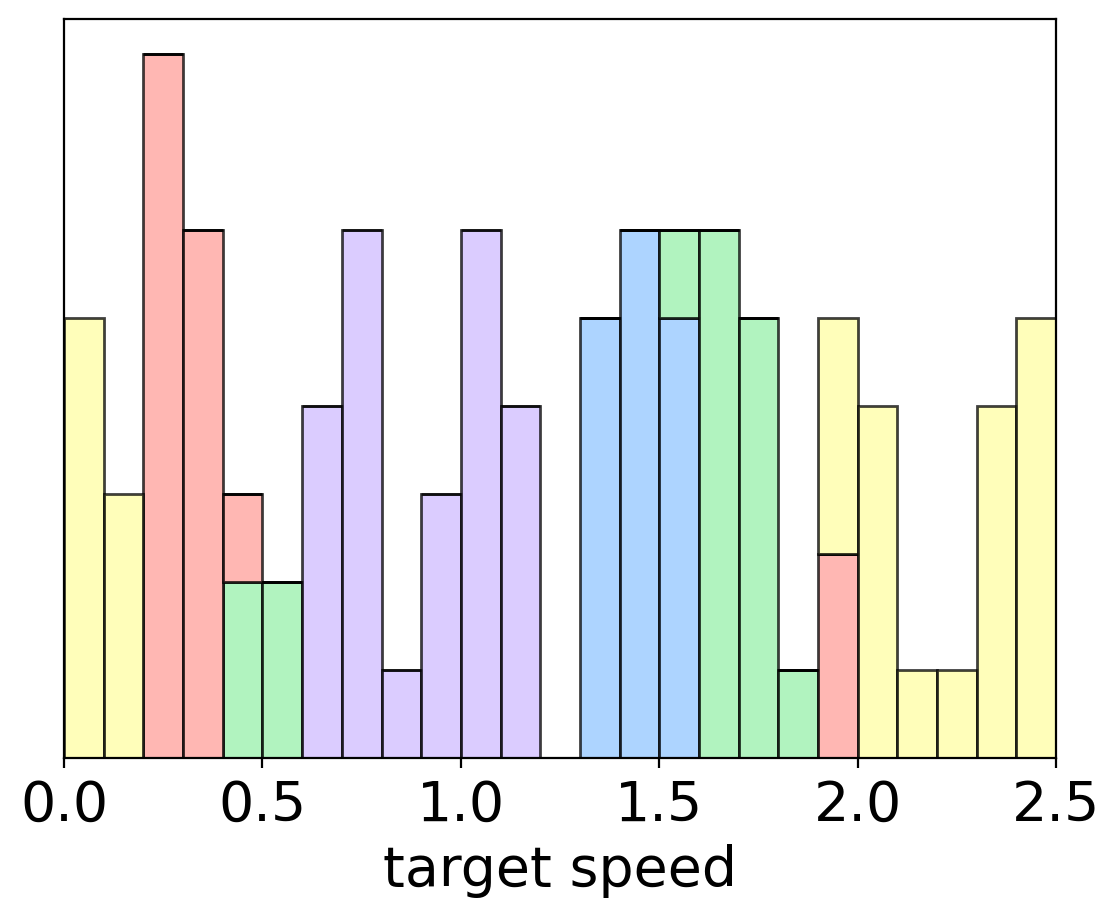
\includegraphics[width=\linewidth]{pics/histograms/end-to-end/Walker2d.png}
    \end{subfigure}\hspace{10pt}%
    \begin{subfigure}{0.3\textwidth}
        \centering
        \caption{Walker2d, cluster (baseline)}
        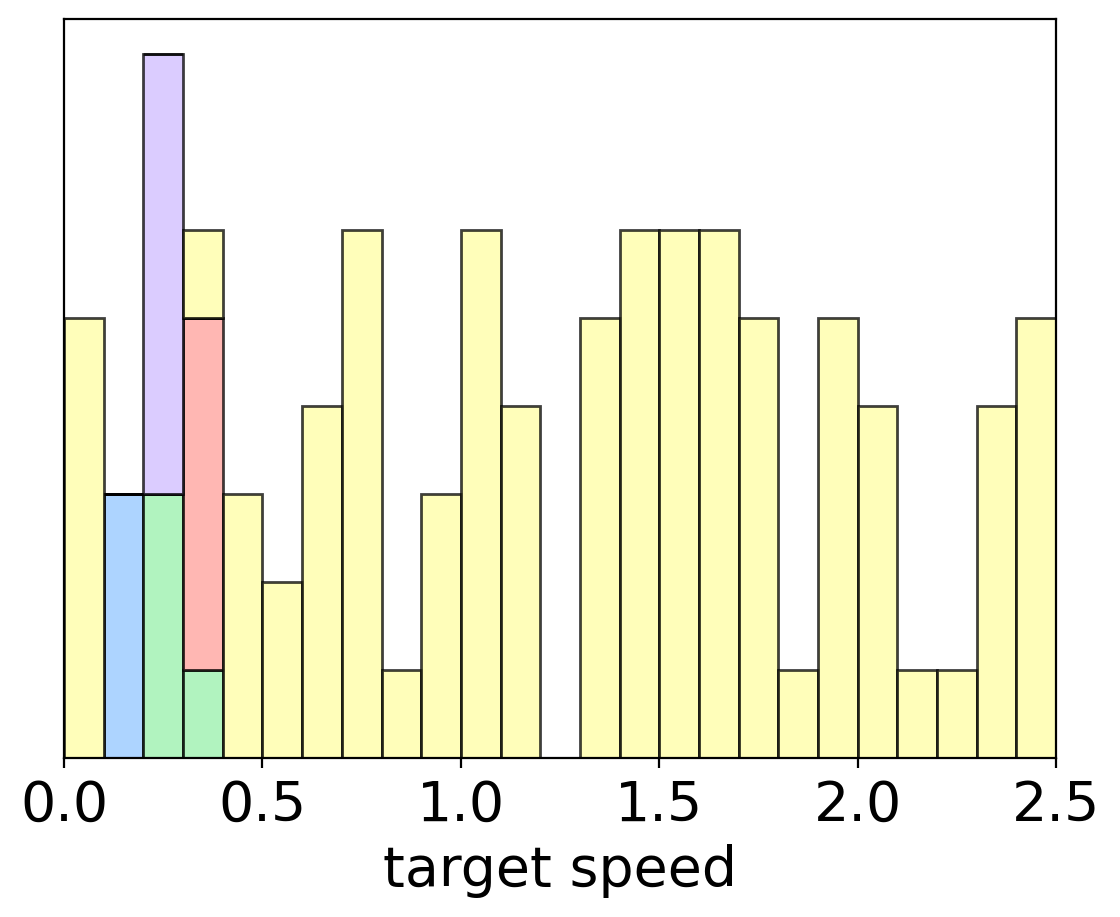
\includegraphics[width=\linewidth]{pics/histograms/cluster/Walker2d.png}
    \end{subfigure}
\caption{Histograms of agent assignments learned by ours and baseline algorithms for $n=100$, $k=5$ in Ant, Hopper, and Walker2d ($0$-th random seed). Each color denotes one of five representatives and bars of this color denote the target velocities of agents assigned to this representative. The expected behavior is a division of the agents' velocities into five intervals of similar sizes, one for each representative.}
\label{fig:results_histograms_app}
\end{center}
\end{figure*}







% \bibliography{main}
% % \bibliographystyle{abbrv}



% \end{document}
